\setcounter{topnumber}{5}
\setcounter{bottomnumber}{5}
\setcounter{totalnumber}{5}

\chapter{Procedimentos e resultados}

\section{Tarefa I}
\subsection{Procedimento}
\begin{description}
  \item[a)]Para iniciar a simula\c{c}\~{a}o de circuitos com o Multisim sugere-se que seja simulado um circuito com tens\~{a}o cont\'{\i}nua e resistores, mostrado na figura 1. Simule o circuito e obtenha os valores solicitados na tabela.\\

\centerline{\begin{minipage}[c]{\textwidth}
\centering
\noindent
        \captionof{figure}{Circuito com tens\~{a}o cont\'{\i}nua a ser simulado.}
		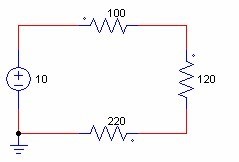
\includegraphics[width=0.5\textwidth]{Imagens/Procedimento1-Imagem1.jpg}
		\legend{Fonte:\cite{MultiSim}}
		\label{fig:image11}
 \end{minipage}}

      Inicialmente simular o circuito da figura 2 e verificar se o diodo est\'{a} em condu\c{c}\~{a}o, al\'{e}m de determinar as grandezas solicitadas na tabela 2.

\centerline{\begin{minipage}[c]{\textwidth}
\centering
\noindent
        \captionof{figure}{Circuito com diodo em condu\c{c}\~{a}o}
		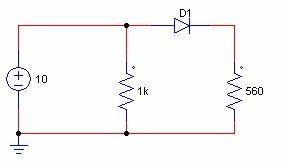
\includegraphics[width=0.5\textwidth]{Imagens/Procedimento1-Imagem2.jpg}
		\legend{Fonte:\cite{MultiSim}}
		\label{fig:image11}
 \end{minipage}}


  \item[b)]A seguir, simule o circuito da figura 3, no qual o diodo deve estar bloqueado. Verifique se isto \'{e} verdadeiro e, al\'{e}m disso, anote as grandezas solicitadas na tabela 3. \\

\centerline{\begin{minipage}[c]{\textwidth}
\centering
\noindent
        \captionof{figure}{Circuito com diodo em condu\c{c}\~{a}o.}
		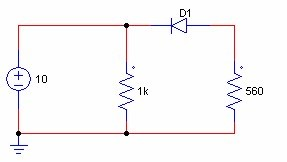
\includegraphics[width=0.5\textwidth]{Imagens/Procedimento1-Imagem3.jpg}
		\legend{Fonte:\cite{MultiSim}}
		\label{fig:image11}
 \end{minipage}}
\end{description}

\subsection{Resultado}
\begin{description}
  \item[a)]A simula\c{c}\~{a}o foi realizada usando o software Multisim, como segue na figura.\\

\centerline{\begin{minipage}[c]{\textwidth}
\centering
\noindent
        \captionof{figure}{Simula\c{c}\~{a}o do circuito 1}
		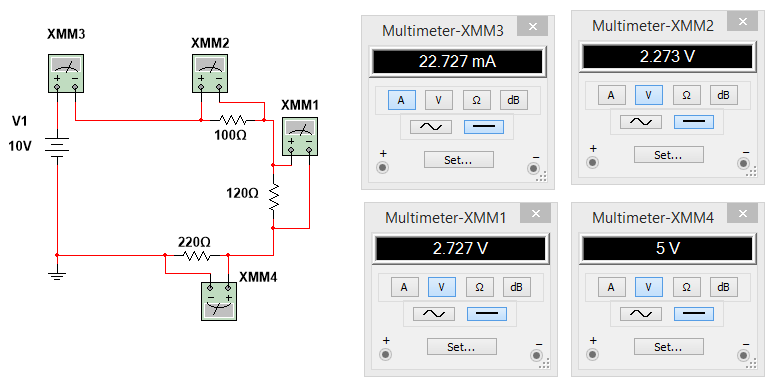
\includegraphics[width=0.5\textwidth]{Imagens/Resultado1-Imagem1.png}
		\legend{Fonte:\cite{MultiSim}}
		\label{fig:image11}
 \end{minipage}}


  A tabela foi constru\'{\i}da com base dos valores da simula\c{c}\~{a}o. \\

  \centerline{\begin{minipage}[c]{\textwidth}
  		\label{tabela1 - gisele}
  		\captionof{table}{Dados do circuito 1 (Simula\c{c}\~{a}o)}
  		\centering
	\begin{tabular}{@{}|c|c|c|@{}}
		\toprule
		\textit{\textbf{Elemento}}         & \textit{\textbf{Grandeza}}      & \textit{\textbf{Valor obtido}} \\ \midrule
		Fonte            & Corrente (mA) & 22,727       \\ \cmidrule(l){2-3}
		& Potencia (W)  & 0,227        \\ \midrule
		& Tens\~{a}o (V)    & 2,273        \\ \cmidrule(l){2-3}
		Resistor de 100$\Omega$ & Pot\^{e}ncia (W)  & 0,052        \\ \cmidrule(l){2-3}
		& Corrente (mA) & 22,727       \\ \midrule
		& Tens\~{a}o (V)    & 2,727        \\ \cmidrule(l){2-3}
		Resistor 120$\Omega$   & Pot\^{e}ncia (W)  & 0,062        \\ \cmidrule(l){2-3}
		& Corrente (mA) & 22,727       \\ \midrule
		& Tens\~{a}o (V)    & 5            \\ \cmidrule(l){2-3}
		Resistor 220$\Omega$   & Pot\^{e}ncia (W)  & 0,114        \\ \cmidrule(l){2-3}
		& Corrente (mA) & 22,727       \\ \bottomrule
	\end{tabular}
  \end{minipage}}
  A pr\'{o}xima tabela refere-se aos dados obtidos com a constru\c{c}\~{a}o do circuito 1. Tal constru\c{c}\~{a}o foi realizada com o aux\'{\i}lio de uma protoboard.
Nota-se que os valores obtidos da corrente de todos os elementos foi o mesmo, isso se deu porque tratava-se de um circuito em s\'{e}rie. A pot\^{e}ncia foi obtida (tanto na simula\c{c}\~{a}o, quanto no experimento) por meio da formula abaixo.\\
\begin{equation}\label{potencia}
  P = U \cdot i
\end{equation}
Onde P \'{e} a pot\^{e}ncia (em Watts), U \'{e} a tens\~{a}o (em Volts) e i \'{e} intensidade de corrente (em Amperes).

  \centerline{\begin{minipage}[c]{\textwidth}
		\label{tabela2 - gisele}
		\captionof{table}{Dados do circuito 1 (Experimento)}
		\centering
			\begin{tabular}{@{}|c|c|c|@{}}
				\toprule
				\textit{\textbf{Elemento}} & \textit{\textbf{Grandeza}} & \textit{\textbf{Valor obtido}} \\ \midrule
				Fonte                      & Corrente (mA)              & 23                             \\ \cmidrule(l){2-3}
				& Potencia (W)               & 0,2                            \\ \midrule
				& Tens\~{a}o (V)                 & 2,269                          \\ \cmidrule(l){2-3}
				Resistor de 100$\Omega$           & Pot\^{e}ncia (W)               & 0,052                          \\ \cmidrule(l){2-3}
				& Corrente (mA)              & 23                             \\ \midrule
				& Tens\~{a}o (V)                 & 2,732                          \\ \cmidrule(l){2-3}
				Resistor 120$\Omega$             & Pot\^{e}ncia (W)               & 0,063                          \\ \cmidrule(l){2-3}
				& Corrente (mA)              & 23                             \\ \midrule
				& Tens\~{a}o (V)                 & 5,013                          \\ \cmidrule(l){2-3}
				Resistor 220$\Omega$             & Pot\^{e}ncia (W)               & 0,115                          \\ \cmidrule(l){2-3}
				& Corrente (mA)              & 23                             \\ \bottomrule
			\end{tabular}
\end{minipage}}

Comparando as Tabelas 1 e 2, constatou-se que os valores obtidos foram muito pr\'{o}ximos e est\~{a}o de acordo com o esperado.



  \item[b)]A simula\c{c}\~{a}o do circuito 2 foi realizada usando o software Multisim, como segue na figura. O diodo em quest\~{a}o est\'{a} polarizado, ou seja, h\'{a} condu\c{c}\~{a}o de corrente. \\

\centerline{\begin{minipage}[c]{\textwidth}
\centering
\noindent
        \captionof{figure}{Simula\c{c}\~{a}o circuito 2}
		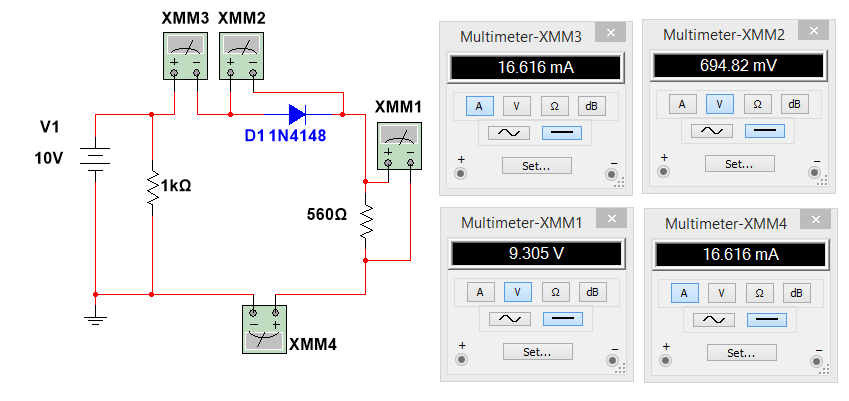
\includegraphics[width=0.5\textwidth]{Imagens/Resultado1-Imagem2.png}
		\legend{Fonte:\cite{MultiSim}}
		\label{fig:image11}
 \end{minipage}}
      Os dados contidos na Tabela 3 foram obtidos com a simula\c{c}\~{a}o do circuito.  \\

        \centerline{\begin{minipage}[c]{\textwidth}
      		\label{tabela3 - gisele}
      		\captionof{table}{Dados do circuito 2 (Simula\c{c}\~{a}o)}
      		\centering
	\begin{tabular}{@{}|c|c|c|@{}}
		\toprule
		\textit{\textbf{Elemento}} & \textit{\textbf{Grandeza}}              & \textit{\textbf{Valor Obtido}} \\ \midrule
		& Estado     (condu\c{c}\~{a}o      ou bloqueado) & Condu\c{c}\~{a}o                       \\ \cmidrule(l){2-3}
		Diodo D1                   & Corrente (mA)                           & 16,616                         \\ \cmidrule(l){2-3}
		& Tens\~{a}o direta (mV)                      & 694,82                         \\ \midrule
		Resistor de 560$\Omega$           & Corrente (mA)                           & 16,616                         \\ \cmidrule(l){2-3}
		& Tens\~{a}o (V)                              & 9,305                          \\ \bottomrule
	\end{tabular}
      \end{minipage}}

      Na Tabela 4 encontram-se os dados obtidos com a constru\c{c}\~{a}o do circuito 2. Tal constru\c{c}\~{a}o foi realizada com o aux\'{\i}lio de uma protoboard. \\

            \centerline{\begin{minipage}[c]{\textwidth}
      		\label{tabela4 - gisele}
      		\captionof{table}{Dados do circuito 2 (experimento)}
      		\centering
	\begin{tabular}{@{}|c|c|c|@{}}
		\toprule
		\textit{\textbf{Elemento}} & \textit{\textbf{Grandeza}}              & \textit{\textbf{Valor Obtido}} \\ \midrule
		& Estado     (condu\c{c}\~{a}o      ou bloqueado) & Condu\c{c}\~{a}o                       \\ \cmidrule(l){2-3}
		Diodo D1                   & Corrente (mA)                           & 17                         \\ \cmidrule(l){2-3}
		& Tens\~{a}o direta (mV)                      & 767                         \\ \midrule
		Resistor de 560$\Omega$           & Corrente (mA)                           & 17                         \\ \cmidrule(l){2-3}
		& Tens\~{a}o (V)                              & 9,25                          \\ \bottomrule
	\end{tabular}
      \end{minipage}}

      \'{E} valido ressaltar neste circuito que os valores da corrente s\~{a}o os mesmo, apesar de o circuito possuir uma resist\^{e}ncia em paralelo, isso se deu porque a corrente sempre “procura” o lugar de menor resist\^{e}ncia para passar, logo, h\'{a} um desvio insignificante de corrente. Ao comparar Tabelas 3 e 4, nota-se que os dados obtidos foram satisfat\'{o}rios ao experimento.

  \item[c)]A simula\c{c}\~{a}o do circuito 3 foi realizada usando o software Multisim, como segue na figura. O diodo encontra-se no estado bloqueado, ou seja, n\~{a}o h\'{a} condu\c{c}\~{a}o de corrente. \\

\centerline{\begin{minipage}[c]{\textwidth}
		\centering
		\noindent
		\captionof{figure}{Simula\c{c}\~{a}o do circuito 3}
		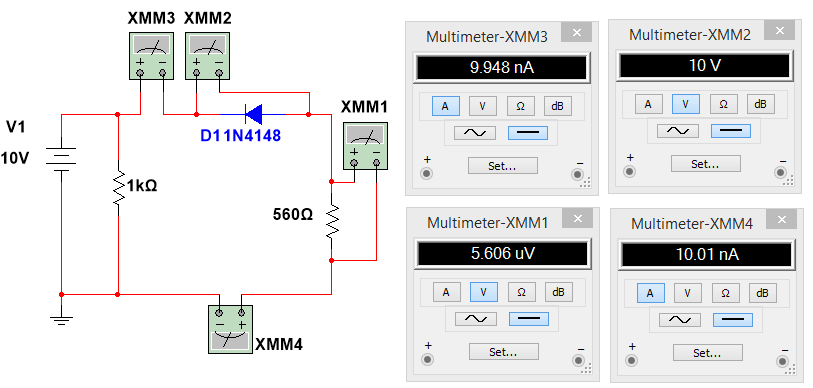
\includegraphics[width=0.5\textwidth]{Imagens/Resultado1-Imagem3.png}
		\legend{Fonte:\cite{MultiSim}}
		\label{fig:image11}
\end{minipage}}

      Os dados abaixo, da tabela 3, foram obtidos com a simula\c{c}\~{a}o do circuito 3. \\

            \centerline{\begin{minipage}[c]{\textwidth}
		\label{tabela5 - gisele}
		\captionof{table}{Dados circuito 3 (Simula\c{c}\~{a}o)}
		\centering
		\begin{tabular}{@{}|c|c|c|@{}}
			\toprule
			\textit{\textbf{Elemento}} & \textit{\textbf{Grandeza}}              & \textit{\textbf{Valor Obtido}} \\ \midrule
			& Estado     (condu\c{c}\~{a}o      ou bloqueado) & Bloqueado                       \\ \cmidrule(l){2-3}
			Diodo D1                   & Corrente (nA)                           & 9,948                         \\ \cmidrule(l){2-3}
			& Tens\~{a}o direta (reversa)                      & 10                         \\ \midrule
			Resistor de 560$\Omega$           & Corrente (nA)                           & 10,01                         \\ \cmidrule(l){2-3}
			& Tens\~{a}o (uV)                              & 5,606                         \\ \bottomrule
		\end{tabular}
\end{minipage}}

      Na tabela abaixo encontram-se os dados obtidos com a constru\c{c}\~{a}o do circuito 3. Tal constru\c{c}\~{a}o foi realizada com o aux\'{\i}lio de uma protoboard. \\

            \centerline{\begin{minipage}[c]{\textwidth}
		\label{tabela6 - gisele}
		\captionof{table}{Dados do circuito 3 (Experimento)}
		\centering
		\begin{tabular}{@{}|c|c|c|@{}}
			\toprule
			\textit{\textbf{Elemento}} & \textit{\textbf{Grandeza}}              & \textit{\textbf{Valor Obtido}} \\ \midrule
			& Estado     (condu\c{c}\~{a}o      ou bloqueado) & Bloqueado                       \\ \cmidrule(l){2-3}
			Diodo D1                   & Corrente                           & 0                         \\ \cmidrule(l){2-3}
			& Tens\~{a}o direta (reversa)                      & 10,02                         \\ \midrule
			Resistor de 560$\Omega$           & Corrente                           & 0                         \\ \cmidrule(l){2-3}
			& Tens\~{a}o                              & 0                         \\ \bottomrule
		\end{tabular}
\end{minipage}}

      Na tabela 5, temos os valores de corrente na ordem de 10-9 ou seja, \'{e} um valor muito pequeno, e experimentalmente na tabela 6, obteve-se tal valor igual a 0, isso se deu devido a precis\~{a}o do Mult\'{\i}metro utilizado. No mais, os valores obtidos foram satisfat\'{o}rios.
\end{description}

\section{Tarefa II}
\subsection{Procedimento}
\noindent Realizar todas as atividades simuladas e compar\'{a}-las com os valores experimentais.

\begin{description}
  \item[a)]Simule o circuito retificador de meia onda mostrado na figura 4 e anote os valores solicitados na tabela 4. \\

\centerline{\begin{minipage}[c]{\textwidth}
		\centering
		\noindent
		\captionof{figure}{Circuito retificador de meia onda}
		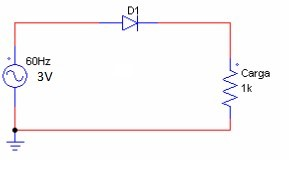
\includegraphics[width=0.5\textwidth]{Imagens/Procedimento2-Imagem1.jpg}
		\legend{Fonte:\cite{MultiSim}}
		\label{fig:image11}
\end{minipage}}

  \item[b)]Desenhe as formas de onda da tens\~{a}o na entrada do retificador (fonte) e ap\'{o}s o diodo, ou seja, na carga.
\end{description}

\subsection{Resultado}
\begin{description}
  \item[a)]A simula\c{c}\~{a}o foi realizada usando o software Multisim, como segue na figura: \\

\centerline{\begin{minipage}[c]{\textwidth}
		\centering
		\noindent
		\captionof{figure}{Simula\c{c}\~{a}o retificador de meia onda}
		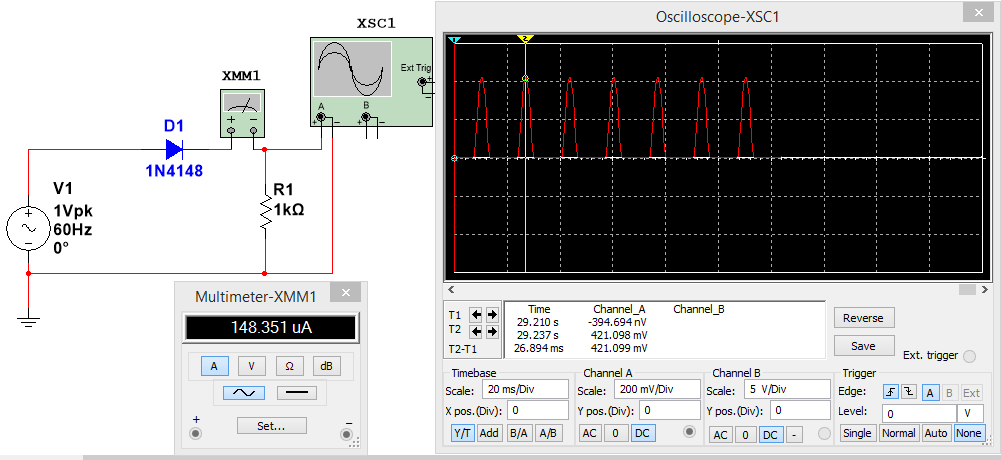
\includegraphics[width=0.5\textwidth]{Imagens/Resultado2-Imagem1.png}
		\legend{Fonte:\cite{MultiSim}}
		\label{fig:image11}
\end{minipage}}

  Para a constru\c{c}\~{a}o da Tabela 7, fez-se uso dos dados da Figura 8. \\

    \centerline{\begin{minipage}[c]{\textwidth}
  		\label{tabela7 - gisele}
  		\captionof{table}{Dados retificador de meia onda (simula\c{c}\~{a}o)}
  		\centering
  			\begin{tabular}{@{}|c|c|c|@{}}
  				\toprule
  				\textit{\textbf{Elemento}} & \textit{\textbf{Grandeza}} & \textit{\textbf{Valor obtido}} \\ \midrule
  				& Tens\~{a}o de pico             & 0,94                           \\ \cmidrule(l){2-3}
  				Fonte                      & Tens\~{a}o eficaz              & 0,664                          \\ \cmidrule(l){2-3}
  				& Tens\~{a}o media               & 0,299                          \\ \midrule
  				Diodo D1                   & Corrente direta media (uA) & 146, 351                       \\ \cmidrule(l){2-3}
  				& Tens\~{a}o reversa m\'{a}xima      & -                              \\ \midrule
  				& Tens\~{a}o m\'{a}xima (mV)         & 421, 098                       \\ \cmidrule(l){2-3}
  				Carga                      & Tens\~{a}o media (mV)          & 131, 328                       \\ \cmidrule(l){2-3}
  				& Corrente media (uA)        & 146, 351                       \\ \bottomrule
  			\end{tabular}
  \end{minipage}}

  Ap\'{o}s a constru\c{c}\~{a}o do circuito, com aux\'{\i}lio do oscilosc\'{o}pio fez-se as seguintes medidas (Figura 9) e montou-se a tabela 8. E a medi\c{c}\~{a}o da correte foi feita usando o mult\'{\i}metro. \\

\centerline{\begin{minipage}[c]{\textwidth}
		\centering
		\noindent
		\captionof{figure}{Retificador de meia onda (Oscilosc\'{o}pio)}
		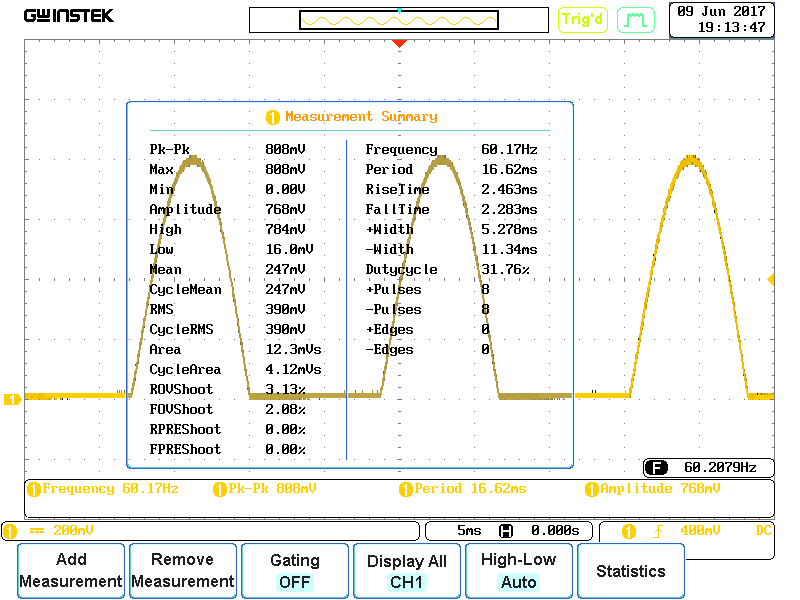
\includegraphics[width=0.5\textwidth]{Imagens/Resultado2-Imagem2.png}
		\legend{Fonte:\cite{Osciloscopio}}
		\label{fig:image11}
\end{minipage}}

    \centerline{\begin{minipage}[c]{\textwidth}
  		\label{tabela8 - gisele}
  		\captionof{table}{Dados Retificador de meia onda (Experimento)}
  		\centering
	\begin{tabular}{@{}|c|c|c|@{}}
		\toprule
		\textit{\textbf{Elemento}} & \textit{\textbf{Grandeza}} & \textit{\textbf{Valor obtido}} \\ \midrule
		& Tens\~{a}o de pico             & 0,94                           \\ \cmidrule(l){2-3}
		Fonte                      & Tens\~{a}o eficaz              & 0,664                          \\ \cmidrule(l){2-3}
		& Tens\~{a}o media               & 0,299                          \\ \midrule
		Diodo D1                   & Corrente direta media (uA) & 136                            \\ \cmidrule(l){2-3}
		& Tens\~{a}o reversa m\'{a}xima      & -                              \\ \midrule
		& Tens\~{a}o m\'{a}xima (mV)         & 404                            \\ \cmidrule(l){2-3}
		Carga                      & Tens\~{a}o media (mV)          & 128,472                        \\ \cmidrule(l){2-3}
		& Corrente media (uA)        & 126                            \\ \bottomrule
	\end{tabular}
  \end{minipage}}

  Comparando os dados da tabela, observa-se que os resultados foram satisfat\'{o}rios. E as discrep\^{a}ncias existentes s\~{a}o devido \`{a} pouca precis\~{a}o do equipamento ou a complica\c{c}\~{o}es no manuseio.
  \item[b)]As formas de ondas de sa\'{\i}da s\~{a}o similares, como representado nas imagens a seguir:\\

\centerline{\begin{minipage}[c]{\textwidth}
		\centering
		\noindent
		\captionof{figure}{Onda de sa\'{\i}da com o simulador}
		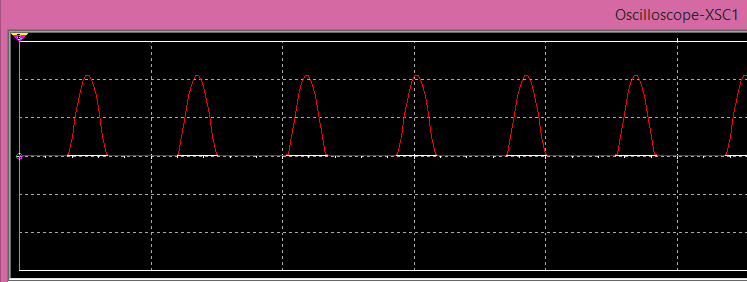
\includegraphics[width=0.5\textwidth]{Imagens/Resultado2-Imagem3.png}
		\legend{Fonte:\cite{MultiSim}}
		\label{fig:image11}
\end{minipage}}


\centerline{\begin{minipage}[c]{\textwidth}
		\centering
		\noindent
		\captionof{figure}{Onda de sa\'{\i}da com o oscilosc\'{o}pio}
		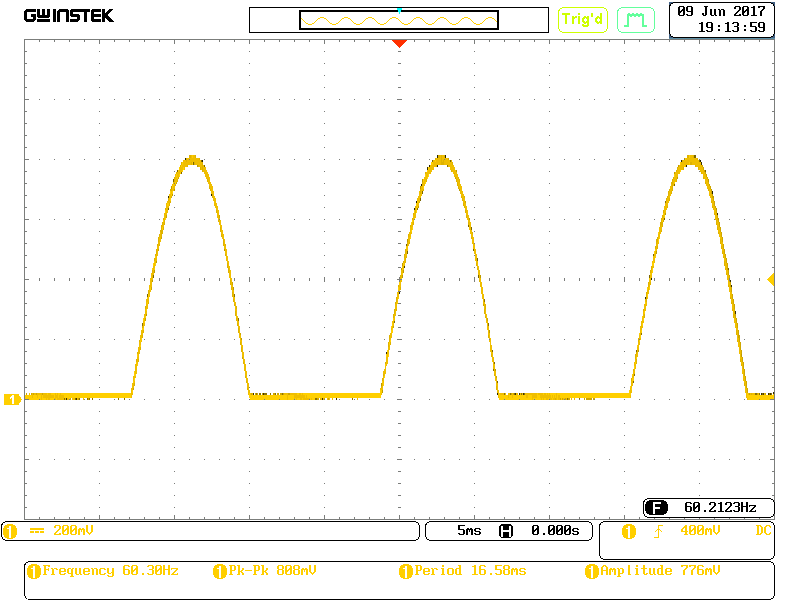
\includegraphics[width=0.5\textwidth]{Imagens/Resultado2-Imagem4.png}
		\legend{Fonte:\cite{Osciloscopio}}
		\label{fig:image11}
\end{minipage}}

  Portanto, obteve-se o resultado esperado.
\end{description}


\section{Tarefa III}
\subsection{Procedimento}
\begin{description}
	\item[a)] Utilize um transformador  de laborat\'{o}rio e me\c{c}a a rela\c{c}\~{a}o de transforma de Vp/Vs = Np/Ns = rela\c{c}\~{a}o de transforma\c{c}\~{a}o, sendo Vp = tens\~{a}o na bobina primaria, Vs = tens\~{a}o na bobina secundaria, Np = numero de espiras na bobina primaria e Ns = numero de espiras na bobina secundaria. Assim antes realizar a simula\c{c}\~{a}o me\c{c}a o valor da tens\~{a}o de sa\'{\i}da do transformador)
	A seguir simule o circuito retificador de onda completa em ponte usando transformador, conforme mostrado na tabela 5. \\
	
\centerline{\begin{minipage}[c]{\textwidth}
		\centering
		\noindent
		\captionof{figure}{Circuito retificador em ponte com transformador.}
		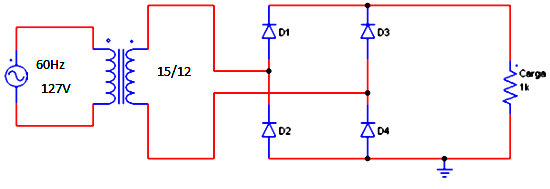
\includegraphics[width=0.5\textwidth]{Imagens/Procedimento4-Imagem1.png}
		\legend{Fonte:\cite{MultiSim}}
		\label{fig:image11}
\end{minipage}}
	
	\item[b)] Desenhe as formas de onda da tens\~{a}o na entrada do retificador (fonte) e ap\'{o}s os diodos, ou seja, na carga.
\end{description}
\subsection{Resultado}

\begin{description}
	\item[a)] Os dados encontrados est\~{a}o na tabela abaixo: \\

	  \centerline{\begin{minipage}[c]{\textwidth}
			\label{tabela1 - paulo}
			\captionof{table}{Dados do circuito retificador onda completa em ponte com transformador.}
			\centering
				\begin{tabular}{@{}|c|c|c|@{}}
					\toprule
					\textit{\textbf{Elemento}} & \textit{\textbf{Grandeza}} & \textit{\textbf{Valor obtido}} \\ \midrule
					& Tens\~{a}o de pico             & 23V                            \\ \cmidrule(l){2-3}
					Prim\'{a}rio de T1             & Tens\~{a}o eficaz              & 15,9V                          \\ \cmidrule(l){2-3}
					& Tens\~{a}o media               & 16,4V                          \\ \midrule
					& Tens\~{a}o de pico             & 18V                            \\ \cmidrule(l){2-3}
					Secund\'{a}rio de T1           & Tens\~{a}o eficaz              & 12,10V                         \\ \cmidrule(l){2-3}
					& Tens\~{a}o media               & 12,72V                         \\ \midrule
					Diodo D1 a D4              & Corrente media direta      & 6,18                           \\ \cmidrule(l){2-3}
					& Tens\~{a}o reversa             & 6,34/6,18/7,31/7,68            \\ \midrule
					& Tens\~{a}o m\'{a}xima              & 22V                            \\ \cmidrule(l){2-3}
					Carga                      & Tens\~{a}o media               & 11V                            \\ \cmidrule(l){2-3}
					& Corrente media(mA)         & 8,27                           \\ \bottomrule
				\end{tabular}
	\end{minipage}}

	\item[b)] As formas de onda est\~{a}o nas imagens abaixo:\\
\centerline{\begin{minipage}[c]{\textwidth}
		\centering
		\noindent
		\captionof{figure}{Onda de entrada (amarela) e onda na carga (azul).}
		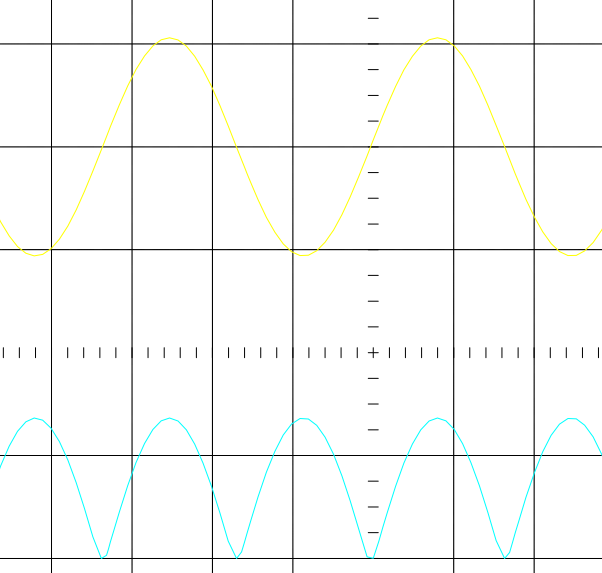
\includegraphics[width=0.5\textwidth]{Imagens/Resultado4-Imagem1.png}
		\legend{Fonte:\cite{MultiSim}}
		\label{fig:image11}
\end{minipage}}

\centerline{\begin{minipage}[c]{\textwidth}
		\centering
		\noindent
		\captionof{figure}{Simula\c{c}\~{a}o do circuito retificador de onda completa}
		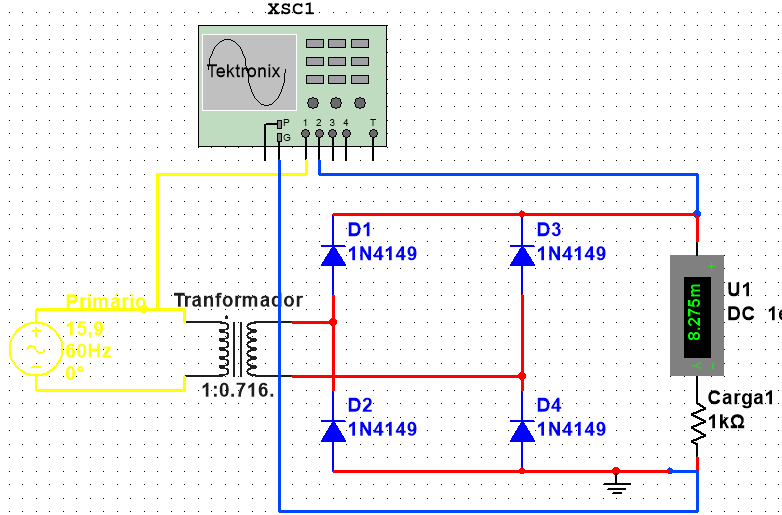
\includegraphics[width=0.5\textwidth]{Imagens/Resultado4-Imagem2.png}
		\legend{Fonte:\cite{MultiSim}}
		\label{fig:image11}
\end{minipage}}

\end{description}


\section{Tarefa IV}
\subsection{Procedimento}
\begin{description}
  \item[a)] O \'{u}ltimo circuito a ser simulado \'{e} o retificador de onda completa usando transformador com deriva\c{c}\~{a}o central (center tap), me\c{c}a a rela\c{c}\~{a}o de transforma\c{c}\~{a}o  de tens\~{a}o entre cada deriva\c{c}\~{a}o, mostrado na figura 6.
Os dados solicitados devem ser anotados na tabela 6. \\

\centerline{\begin{minipage}[c]{\textwidth}
		\centering
		\noindent
		\captionof{figure}{Circuito retificador de onda completa com tap central. }
		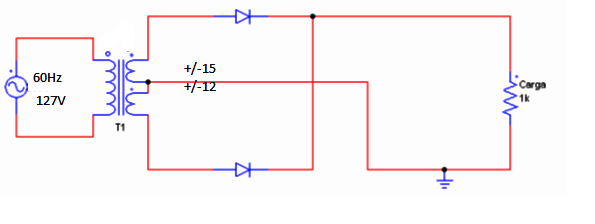
\includegraphics[width=0.5\textwidth]{Imagens/ProcedimentoG-Imagem1.png}
		\legend{Fonte:\cite{MultiSim}}
		\label{fig:image11}
\end{minipage}}


  \item[b)] Desenhe as formas de onda da tens\~{a}o na entrada do retificador (fonte) e ap\'{o}s os diodos, ou seja, na carga. Desenhe tamb\'{e}m a forma de onda da tens\~{a}o sobre o diodo D1.
\end{description}

\subsection{Resultado}

\begin{description}
  \item[a)] Os dados encontrados est\~{a}o nas tabelas abaixo:

  \centerline{\begin{minipage}[c]{\textwidth}
  		\label{tabela1 - gisele}
  		\captionof{table}{Dados do circuito 1 (Simula\c{c}\~{a}o)}
  		\centering
\begin{tabular}{@{}|c|c|c|@{}}
\toprule
\textit{\textbf{Elemento}} & \textit{\textbf{Grandeza}} & \textit{\textbf{Valor obtido}} \\ \midrule
                           & Tens\~{a}o de pico             & Igual a quest\~{a}o anterior       \\ \cmidrule(l){2-3}
Prim\'{a}rio de T1             & Tens\~{a}o eficaz              &                                \\ \cmidrule(l){2-3}
                           & Tens\~{a}o media               & 0                              \\ \midrule
                           & Tens\~{a}o de pico (V)         & 1,15                           \\ \cmidrule(l){2-3}
Secund\'{a}rio 1 de T1         & Tens\~{a}o eficaz (V)          & 0,81                           \\ \cmidrule(l){2-3}
                           & Tens\~{a}o media (V)           & 0,730                          \\ \midrule
                           & Tens\~{a}o de pico (V)         & 1,15                           \\ \cmidrule(l){2-3}
Secund\'{a}rio 2 de T1         & Tens\~{a}o eficaz (V)          & 0,81                           \\ \cmidrule(l){2-3}
                           & Tens\~{a}o media (V)           & 0,729                          \\ \midrule
Diodo D1 a D4              & Corrente media direta      & $350,8 \cdot 10^{-6}$  \\ \cmidrule(l){2-3}
                           & Tens\~{a}o reversa             & -0,78                          \\ \midrule
                           & Tens\~{a}o m\'{a}xima (V)          & 1,08                           \\ \cmidrule(l){2-3}
Carga                      & Tens\~{a}o media (V)           & 0,68                           \\ \cmidrule(l){2-3}
                           & Corrente media (A)         & $702 \cdot 10^{-6}$    \\ \bottomrule
\end{tabular}		
  \end{minipage}}


  \centerline{\begin{minipage}[c]{\textwidth}
		\label{tabelaalgumacoisa - gabriel}
		\captionof{table}{Dados do circuito 1 (Simula\c{c}\~{a}o)}
		\centering
	\begin{tabular}{@{}|c|c|c|@{}}
		\toprule
		\textit{\textbf{Elemento}} & \textit{\textbf{Grandeza}} & \textit{\textbf{Valor obtido}} \\ \midrule
		& Tens\~{a}o de pico (V)         & 120                            \\ \cmidrule(l){2-3}
		Prim\'{a}rio de t1             & Tens\~{a}o eficaz (V)          & 84,85                          \\ \cmidrule(l){2-3}
		& Tens\~{a}o media (V)           & 0                              \\ \midrule
		& Tens\~{a}o de pico (V)         & 1,3                            \\ \cmidrule(l){2-3}
		Secund\'{a}rio 1 de T1         & Tens\~{a}o eficaz (V)          & 0,91                           \\ \cmidrule(l){2-3}
		& Tens\~{a}o media (V)           & 0.83                           \\ \midrule
		& Tens\~{a}o de pico (V)         & 1.3                            \\ \cmidrule(l){2-3}
		Secund\'{a}rio 2 de T1         & Tens\~{a}o eficaz (V)          & 0,91                           \\ \cmidrule(l){2-3}
		& Tens\~{a}o media (V)           & 0.83                           \\ \midrule
		Diodo D1 a D4              & Corrente media direta (V)  & $308 \cdot 10^{-6}$  \\ \cmidrule(l){2-3}
		& Tens\~{a}o reversa (V)         & -0.83                          \\ \midrule
		& Tens\~{a}o m\'{a}xima (V)          & $711 \cdot 10^{-3}$  \\ \cmidrule(l){2-3}
		Carga                      & Tens\~{a}o media (V)           & 0.45                           \\ \cmidrule(l){2-3}
		& Corrente media             & $452 \cdot 10^{-6}$  \\ \bottomrule
	\end{tabular}
\end{minipage}}

  \item[b)] As formas de onda observadas no simulador est\~{a}o nas imagens abaixo: \\

\centerline{{\begin{minipage}[b]{0.4\textwidth}
    \centering
    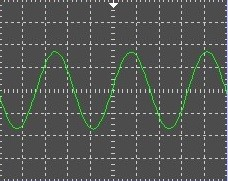
\includegraphics[width=\textwidth]{Imagens/Resultado4-Imagem1.jpg}
    \captionof{figure}{Fonte}
    \legend{Fonte:\cite{MultiSim}}
  \end{minipage}
  \hfill
  \begin{minipage}[b]{0.4\textwidth}
    \centering
    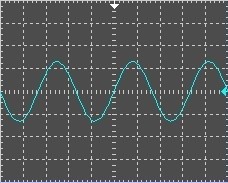
\includegraphics[width=\textwidth]{Imagens/Resultado4-Imagem2.jpg}
    \captionof{figure}{Secund\'{a}rio (T1)}
    \legend{Fonte:\cite{MultiSim}}
  \end{minipage}}
    \begin{minipage}[b]{0.4\textwidth}
    \centering
    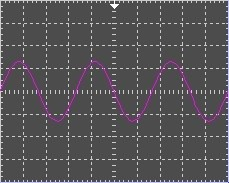
\includegraphics[width=\textwidth]{Imagens/Resultado4-Imagem3.jpg}
    \captionof{figure}{Secund\'{a}rio (T2)}
    \legend{Fonte:\cite{MultiSim}}
  \end{minipage}}
    \begin{minipage}[b]{0.4\textwidth}
    \centering
    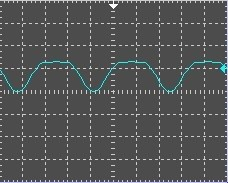
\includegraphics[width=\textwidth]{Imagens/Resultado4-Imagem4.jpg}
    \captionof{figure}{Diodo (D1)}
    \legend{Fonte:\cite{MultiSim}}
  \end{minipage}
    \begin{minipage}[b]{0.4\textwidth}
    \centering
    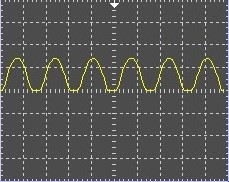
\includegraphics[width=\textwidth]{Imagens/Resultado4-Imagem5.jpg}
    \captionof{figure}{Carga}
    \legend{Fonte:\cite{MultiSim}}
  \end{minipage}

\end{description}

\section{Tarefa V}
\subsection{Procedimento}
Aplicar na bobina primaria do transformador um sinal com o gerador de fun\c{c}\~{o}es com frequ\^{e}ncia de 60Hz, 1kHz e 10kHz, 100kHz com amplitude de 3 Volts, me\c{c}a os valores de amplitude de tens\~{a}o na bobina secundaria do transformador e preencha a tabela 7 (comente os resultados obtidos).
\subsection{Resultado}
Primeiramente, o gerador de fun\c{c}\~{o}es foi ligado diretamente no oscilosc\'{o}pio, para que a tens\~{a}o e frequ\^{e}ncia pudessem ser ajustadas de forma precisa para os valores desejados. Ap\'{o}s ajustados os valores, o gerador de fun\c{c}\~{o}es foi ligado na entrada da bobina prim\'{a}ria, e a sa\'{\i}da da bobina secund\'{a}ria foi ligada no oscilosc\'{o}pio para a an\'{a}lise de onda. O mesmo procedimento foi realizado para todas as frequ\^{e}ncias desejadas. Com a bobina secund\'{a}ria ligada no oscilosc\'{o}pio, foram medidas as tens\~{o}es para cada uma das frequ\^{e}ncias abaixo e para as formas de ondas senoidal e quadrada: \\

  \centerline{\begin{minipage}[c]{\textwidth}
		\label{tabela1 - paolo}
		\captionof{table}{Dados obtidos no oscilosc\'{o}pio}
		\centering
	\begin{tabular}{@{}|c|c|c|@{}}
		\toprule
		\textit{\textbf{Frequ\^{e}ncia}} & \textit{\textbf{Senoidal}} & \textit{\textbf{Quadrada}} \\ \midrule
		60Hz                         & 6,56                       & 6,52                       \\ \midrule
		1kHz                         & 6,88                       & 6,88                       \\ \midrule
		10kHz                        & 6,76                       & 6,84                       \\ \midrule
		100kHz                       & 6,64                       & 6,68                       \\ \bottomrule
	\end{tabular}
\end{minipage}}
Percebe-se que os valores de tens\~{a}o resultante para todas as frequ\^{e}ncias est\~{a}o bastante pr\'{o}ximos, e que todas as frequ\^{e}ncias resultantes s\~{a}o muito pr\'{o}ximas de 60 Hz. Logo, fica bem demonstrado o funcionamento do transformador, o qual para todas as formas de entrada na bobina prim\'{a}ria, gerou uma mesma sa\'{\i}da na bobina secund\'{a}ria. \\

Abaixo, temos as formas de onda obtidas para cada medi\c{c}\~{a}o: \\

%%%%%% 60 Hz
\centerline{{\begin{minipage}[b]{0.48\textwidth}
			\centering
			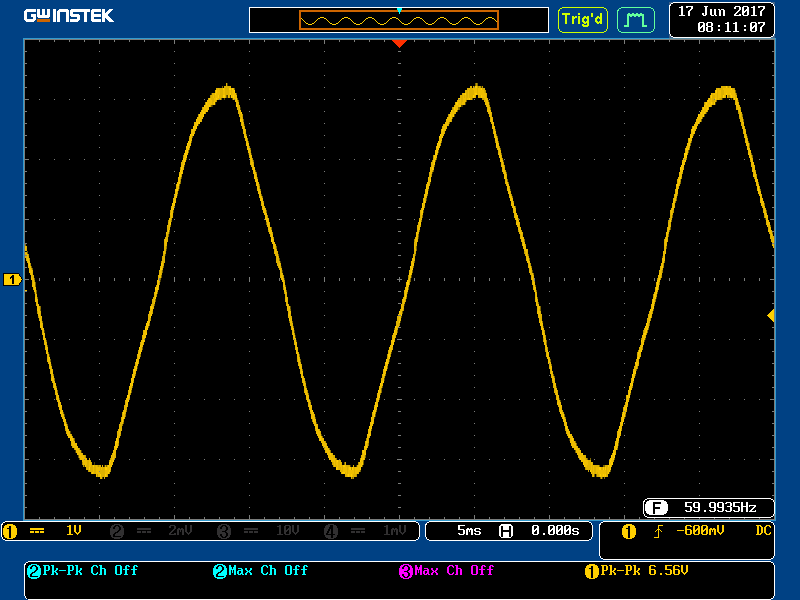
\includegraphics[width=\textwidth]{Imagens/Resultados5-Imagem03(Senoidal1).png}
			\captionof{figure}{60 Hz - Senoidal}
			\legend{Fonte:\cite{Osciloscopio}}
		\end{minipage}
		\hfill
		\begin{minipage}[b]{0.48\textwidth}
			\centering
			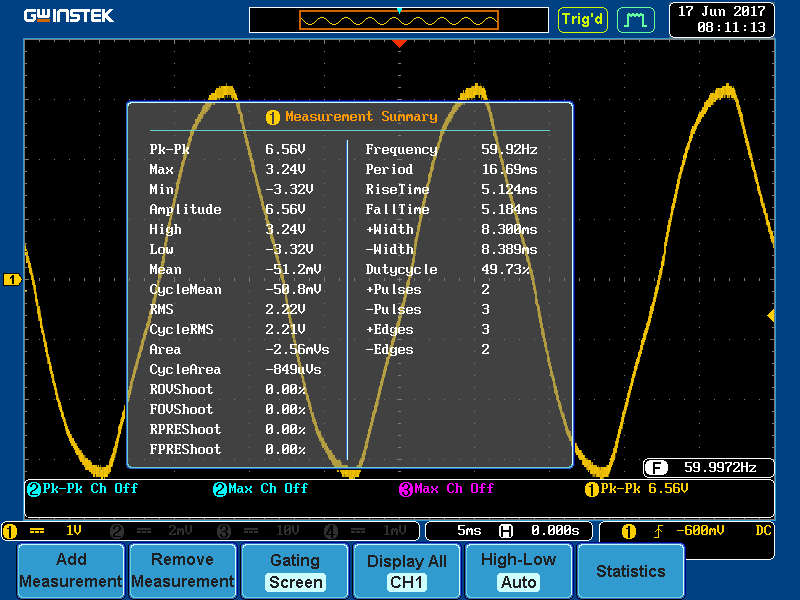
\includegraphics[width=\textwidth]{Imagens/Resultados5-Imagem04(Senoidal2).png}
			\captionof{figure}{60 Hz - Senoidal}
			\legend{Fonte:\cite{Osciloscopio}}
	\end{minipage}}}

 %%%%%%%%%%%%
\centerline{{\begin{minipage}[b]{0.48\textwidth}
			\centering
			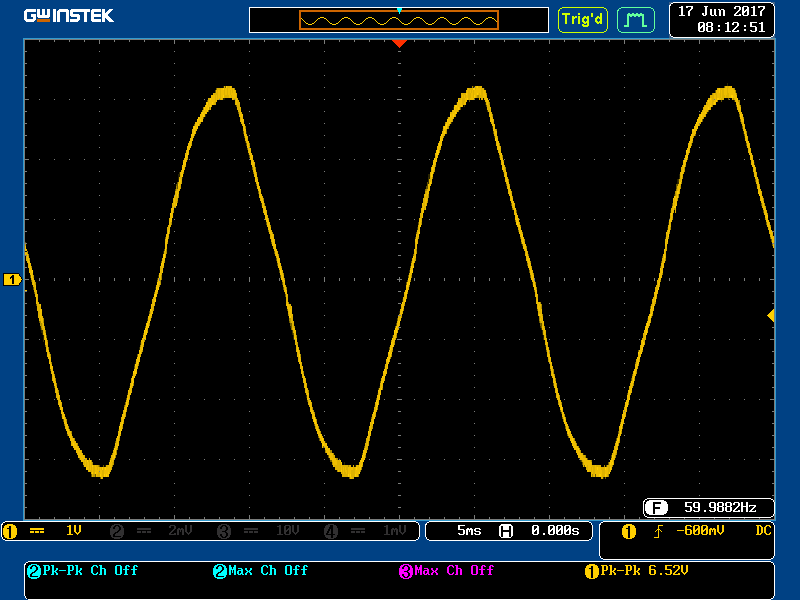
\includegraphics[width=\textwidth]{Imagens/Resultados5-Imagem01(Quadrada01).png}
			\captionof{figure}{60 Hz - Quadrada}
			\legend{Fonte:\cite{Osciloscopio}}
		\end{minipage}
		\hfill
		\begin{minipage}[b]{0.48\textwidth}
			\centering
			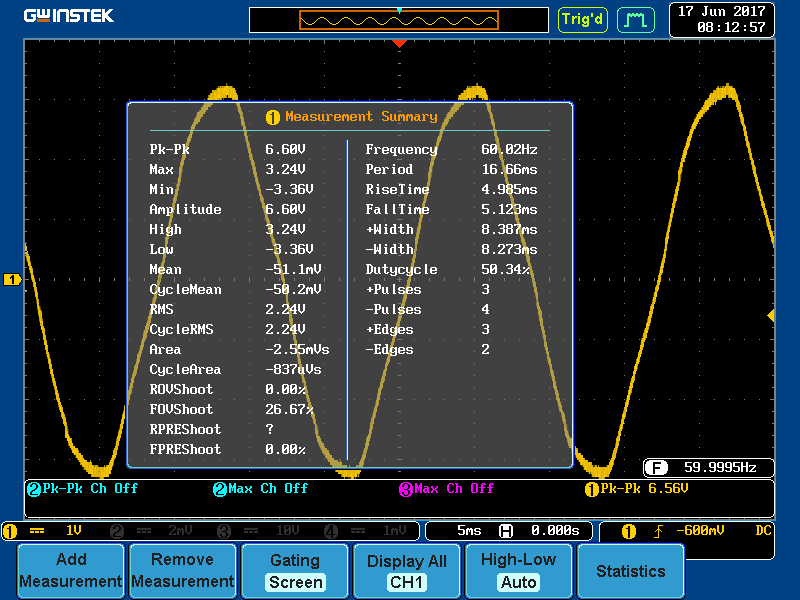
\includegraphics[width=\textwidth]{Imagens/Resultados5-Imagem02(Quadrada02).png}
			\captionof{figure}{60 Hz - Quadrada}
			\legend{Fonte:\cite{Osciloscopio}}
\end{minipage}}}


%%%%%%%%%%%%%%%
\centerline{{\begin{minipage}[b]{0.48\textwidth}
			\centering
			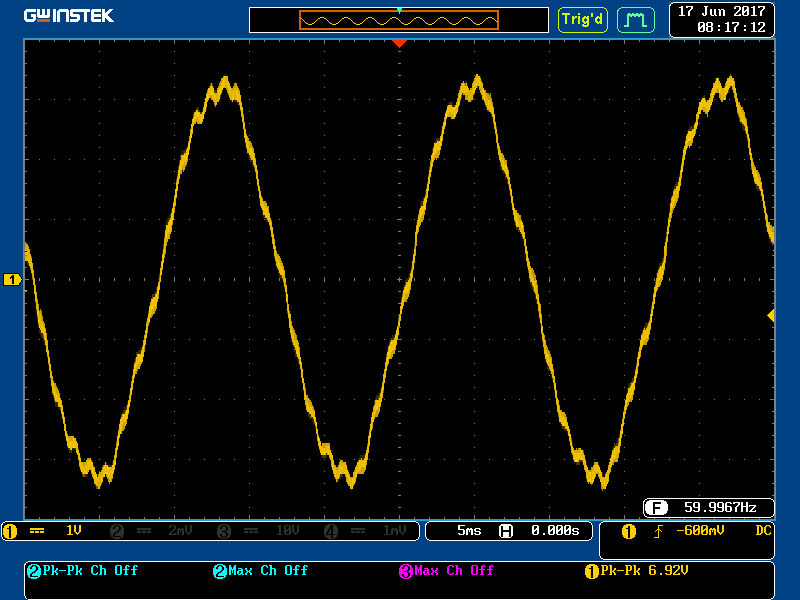
\includegraphics[width=\textwidth]{Imagens/Resultados5-Imagem07(Senoidal3).png}
			\captionof{figure}{1 kHz - Senoidal}
			\legend{Fonte:\cite{Osciloscopio}}
		\end{minipage}
		\hfill
		\begin{minipage}[b]{0.48\textwidth}
			\centering
			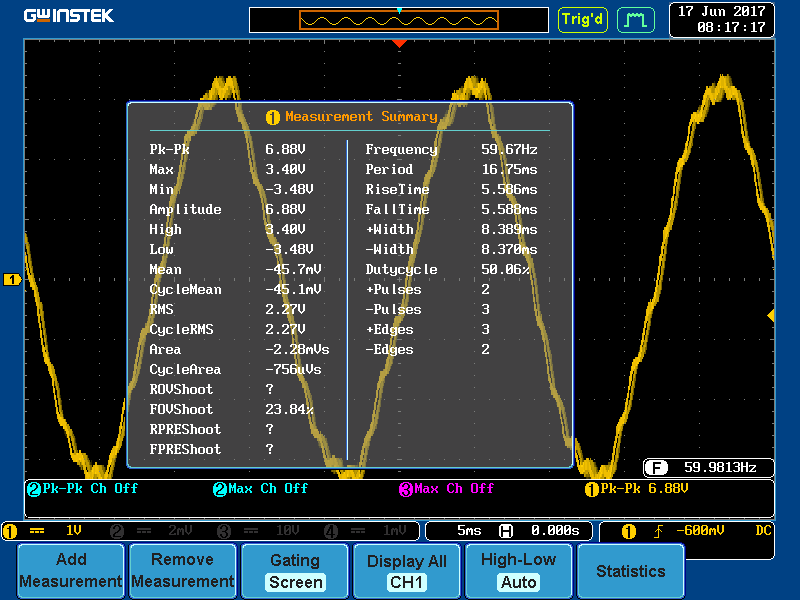
\includegraphics[width=\textwidth]{Imagens/Resultados5-Imagem08(Senoidal4).png}
			\captionof{figure}{1 kHz - Senoidal}
			\legend{Fonte:\cite{Osciloscopio}}
\end{minipage}}}

%%%%%%%%%%%%%
\centerline{{\begin{minipage}[b]{0.48\textwidth}
			\centering
			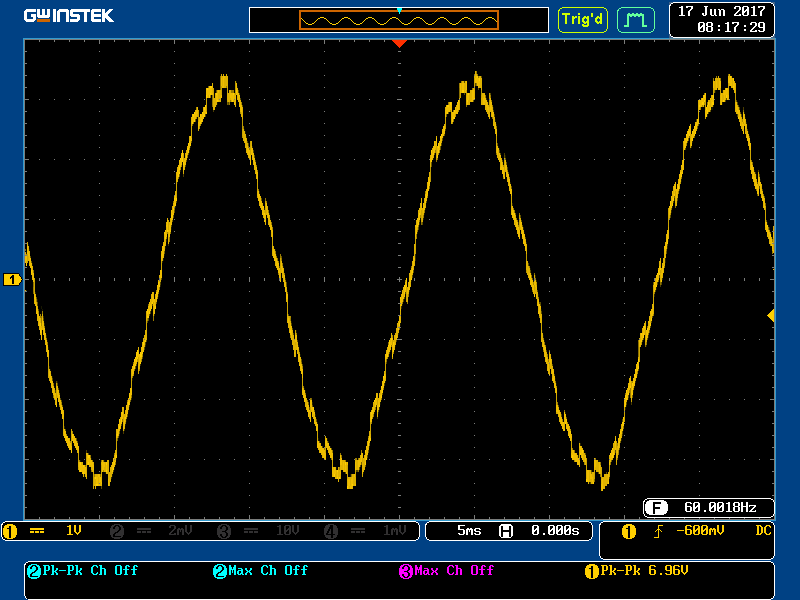
\includegraphics[width=\textwidth]{Imagens/Resultados5-Imagem05(Quadrada03).png}
			\captionof{figure}{1 kHz - Quadrada}
			\legend{Fonte:\cite{Osciloscopio}}
		\end{minipage}
		\hfill
		\begin{minipage}[b]{0.48\textwidth}
			\centering
			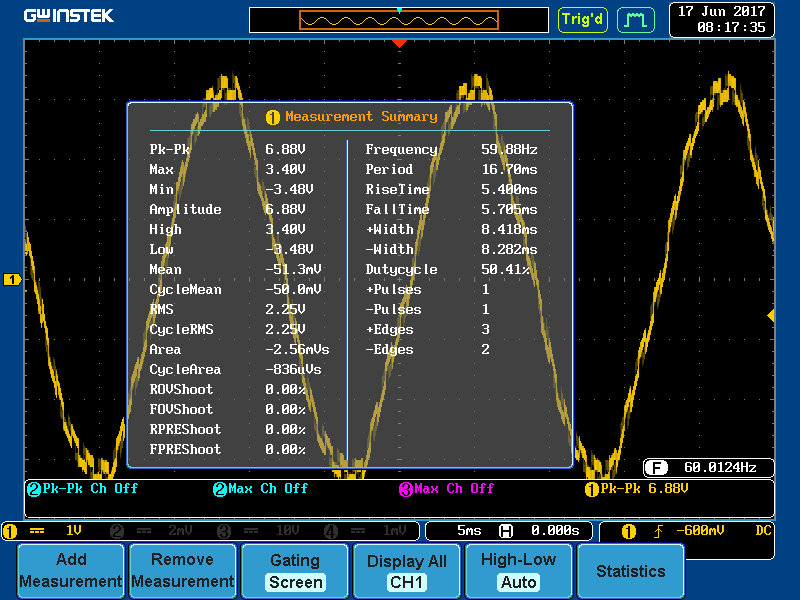
\includegraphics[width=\textwidth]{Imagens/Resultados5-Imagem06(Quadrada04).png}
			\captionof{figure}{1 kHz - Quadrada}
			\legend{Fonte:\cite{Osciloscopio}}
\end{minipage}}}

%%%%%%%%%%%%%%%
\centerline{{\begin{minipage}[b]{0.48\textwidth}
			\centering
			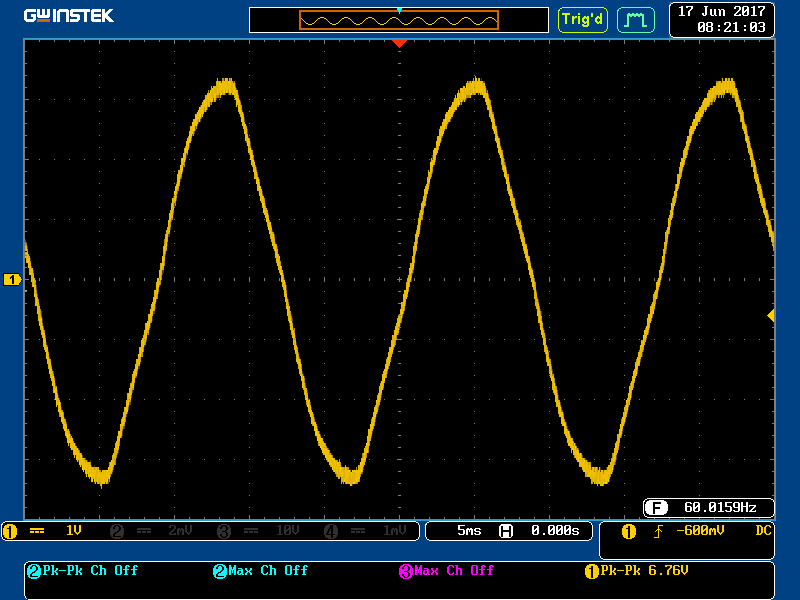
\includegraphics[width=\textwidth]{Imagens/Resultados5-Imagem11(Senoidal5).png}
			\captionof{figure}{10 kHz - Senoidal}
			\legend{Fonte:\cite{Osciloscopio}}
		\end{minipage}
		\hfill
		\begin{minipage}[b]{0.48\textwidth}
			\centering
			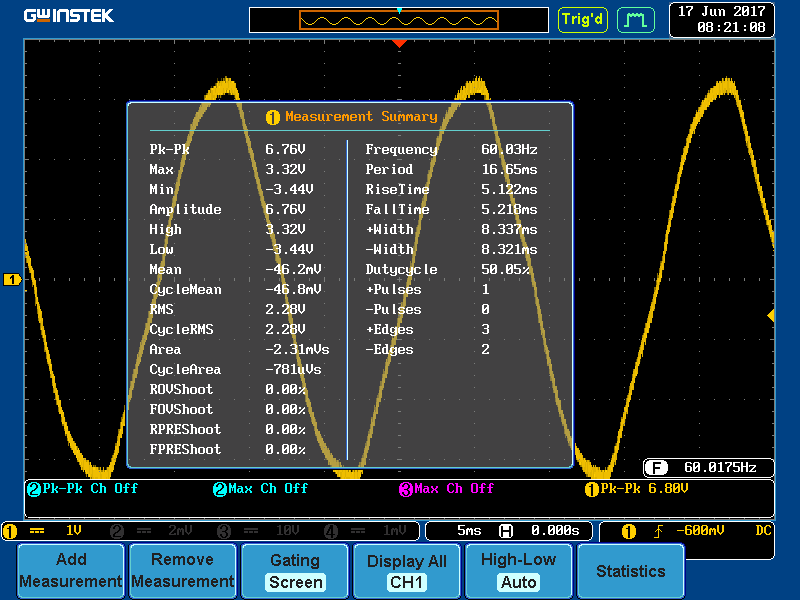
\includegraphics[width=\textwidth]{Imagens/Resultados5-Imagem12(Senoidal6).png}
			\captionof{figure}{10 kHz - Senoidal}
			\legend{Fonte:\cite{Osciloscopio}}
\end{minipage}}}

\centerline{{\begin{minipage}[b]{0.48\textwidth}
			\centering
			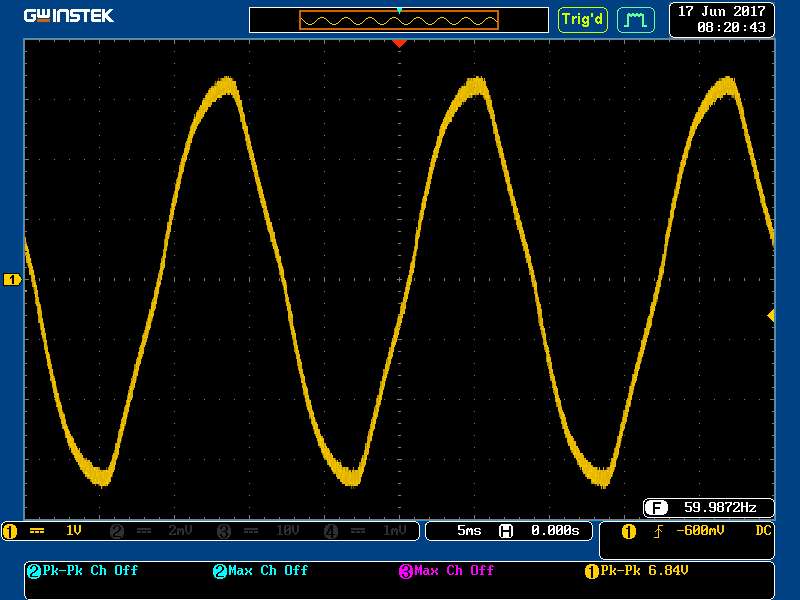
\includegraphics[width=\textwidth]{Imagens/Resultados5-Imagem09(Quadrada05).png}
			\captionof{figure}{10 kHz - Quadrada}
			\legend{Fonte:\cite{Osciloscopio}}
		\end{minipage}
		\hfill
		\begin{minipage}[b]{0.48\textwidth}
			\centering
			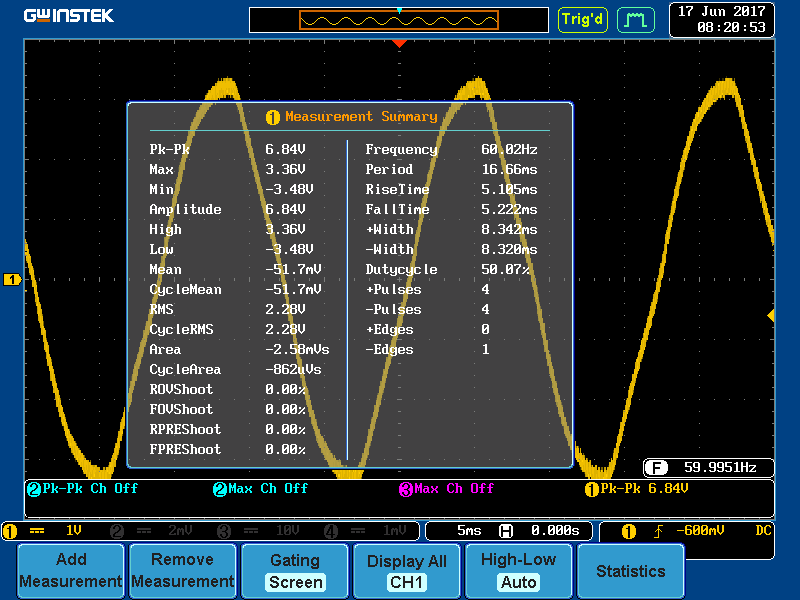
\includegraphics[width=\textwidth]{Imagens/Resultados5-Imagem10(Quadrada06).png}
			\captionof{figure}{10 kHz - Quadrada}
			\legend{Fonte:\cite{Osciloscopio}}
\end{minipage}}}

\centerline{{\begin{minipage}[b]{0.48\textwidth}
			\centering
			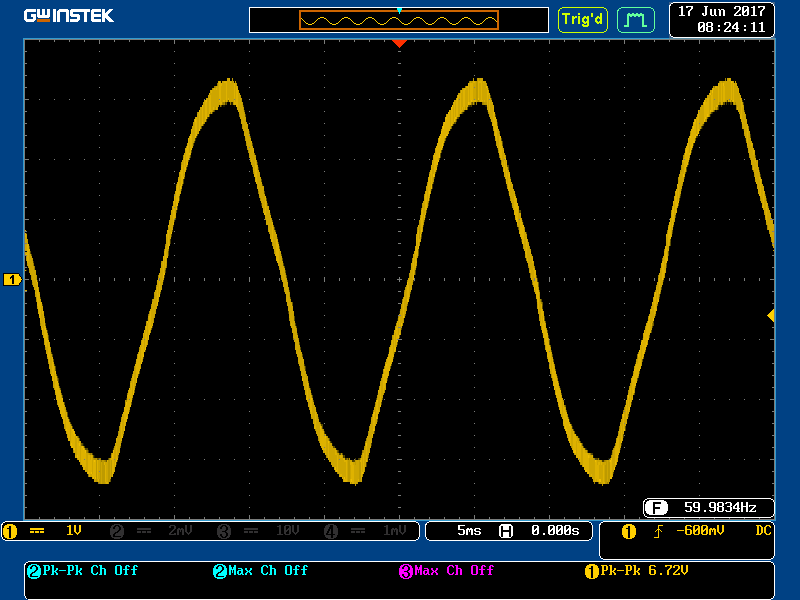
\includegraphics[width=\textwidth]{Imagens/Resultados5-Imagem15(Senoidal7).png}
			\captionof{figure}{100 kHz - Senoidal}
			\legend{Fonte:\cite{Osciloscopio}}
		\end{minipage}
		\hfill
		\begin{minipage}[b]{0.48\textwidth}
			\centering
			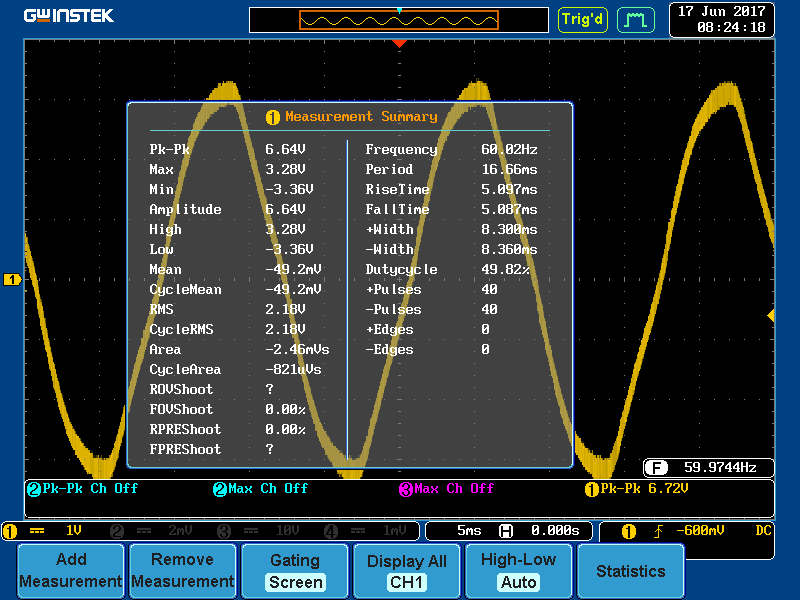
\includegraphics[width=\textwidth]{Imagens/Resultados5-Imagem16(Senoidal8).png}
			\captionof{figure}{100 kHz - Senoidal}
			\legend{Fonte:\cite{Osciloscopio}}
\end{minipage}}}

\centerline{{\begin{minipage}[b]{0.48\textwidth}
			\centering
			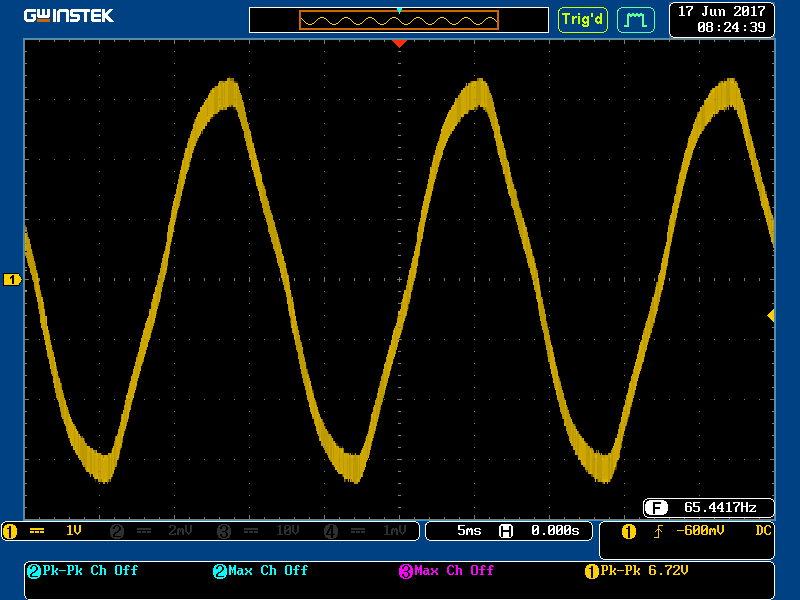
\includegraphics[width=\textwidth]{Imagens/Resultados5-Imagem13(Quadrada07).png}
			\captionof{figure}{100 kHz - Quadrada}
			\legend{Fonte:\cite{Osciloscopio}}
		\end{minipage}
		\hfill
		\begin{minipage}[b]{0.48\textwidth}
			\centering
			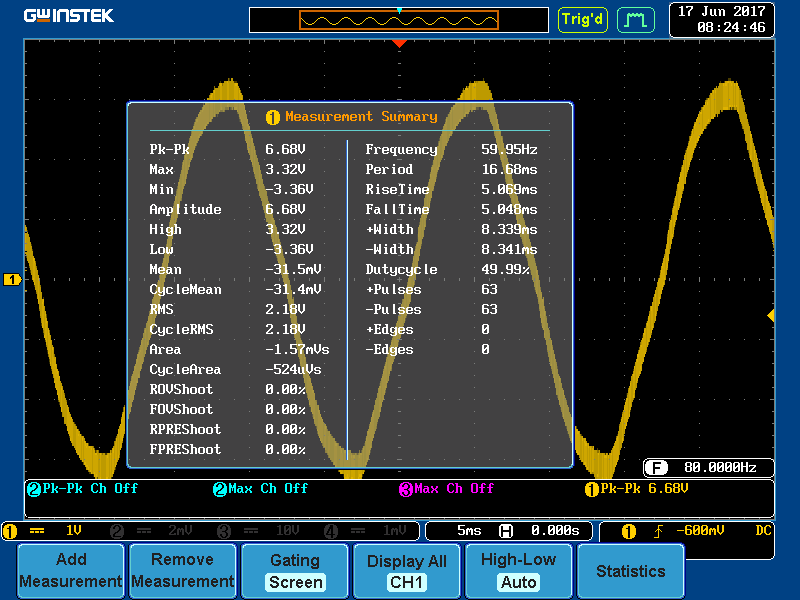
\includegraphics[width=\textwidth]{Imagens/Resultados5-Imagem14(Quadrada08).png}
			\captionof{figure}{100 kHz - Quadrada}
			\legend{Fonte:\cite{Osciloscopio}}
\end{minipage}}}